\documentclass[fleqn, 10pt]{article}

% Paquetes necesarios
\usepackage[utf8]{inputenc}
\usepackage[english]{babel}
\usepackage{amsthm, amsmath}
\usepackage{nccmath} %Para centrar ecuaciones
\usepackage{graphicx}
\graphicspath{ {Documentos/} }
\usepackage{tikz}
\usepackage{amssymb}
\usepackage[linesnumbered]{whilecode2}

% Personalizo mi alfabeto
\DeclareMathAlphabet{\pazocal}{OMS}{zplm}{m}{n}
\newcommand{\Lb}{\pazocal{L}}

% Definimos los entornos para definiciones, teoremas, etc...
\theoremstyle{plain}
\newtheorem{proposicion}{Proposición}

\theoremstyle{definition}
\newtheorem{definition}{Definición}[section]
\newtheorem{example}{Ejemplo}[section]

%Definimos el título
\title{Teoría de Autómatas y Lenguajes Formales\\[.4\baselineskip]Práctica 3}
\author{Irene, Recio López}
\date{\today}

%Comienzo del documento
\begin{document}

%Generamos el título
\maketitle

\subsubsection*{Ejercicio 1: Prove that the function add(x,y) = x + y, with x, y $\in$ $\mathbb{N}$ is Turing-computable using the unary notation $|$ . You have to create a TM wth two arguments separated by a blank symbol that starts and ends behind the stings}
(Recorriendo el string de izquierda a derecha)

\begin{table}[h!]
\begin{tabular}{c c c c}
$q_0$ & $*$ & $r$  & $q_1$
\\
$q_0$ & $|$ & $|$  & $q_0$
\\
\hline
$q_1$ & $*$ & $|$  & $q_2$
\\
$q_1$ & $|$ & $r$  & $q_1$
\\
\hline
$q_2$ & $*$ & $r$  & $q_3$
\\
$q_2$ & $|$ & $l$  & $q_2$
\\
\hline
$q_3$ & $*$ & $*$  & $q_4$
\\
$q_3$ & $|$ & $*$  & $q_3$
\\
\hline
$q_4$ & $*$ & $r$  & $q_4$
\\
$q_4$ & $|$ & $*$  & $q_5$
\\
\hline
$q_5$ & $*$ & $*$  & $q_5$
\\
$q_5$ & $|$ & $h$  & $q_5$
\\
\end{tabular}
\end{table}
\begin{center}
Máquina de Turing diseñado con JFLAP
\\
	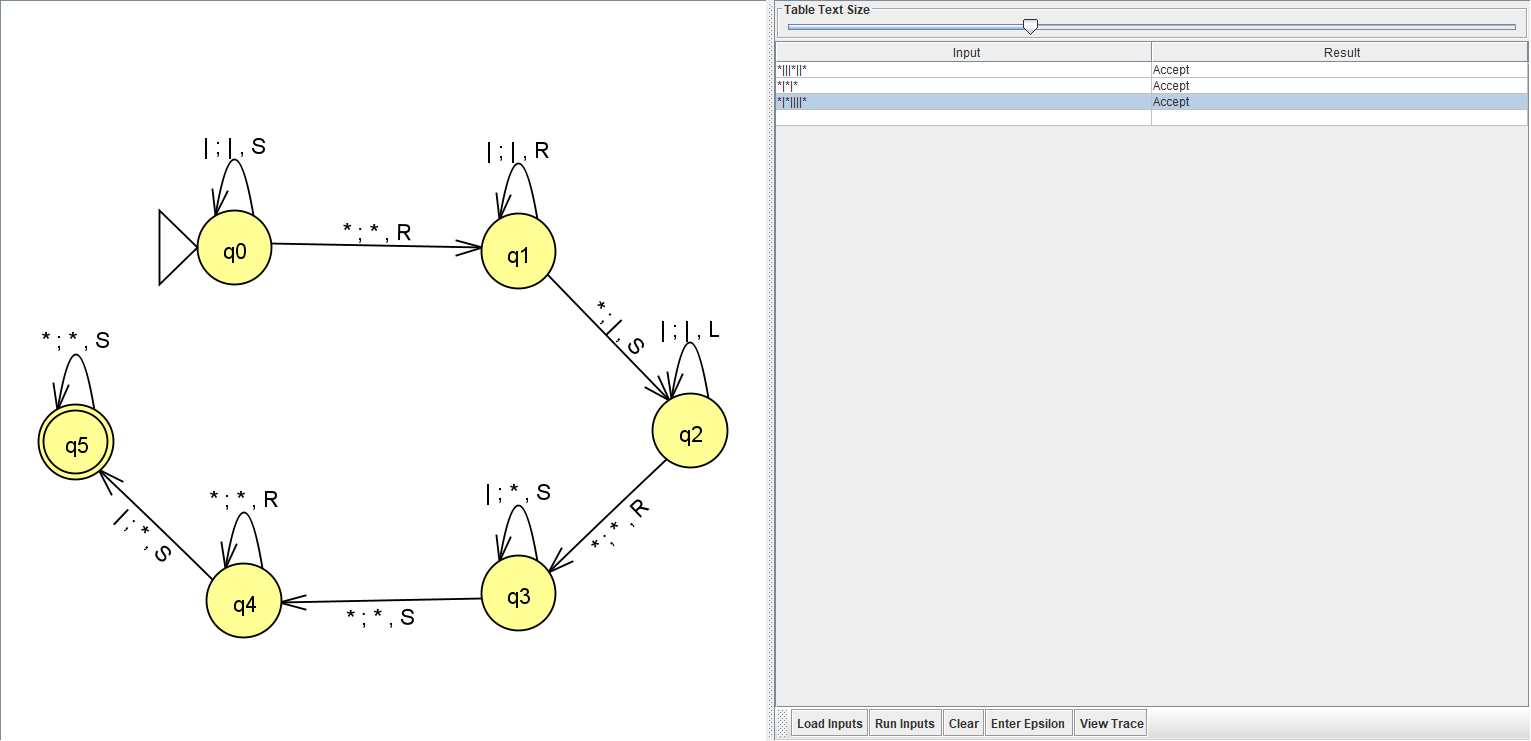
\includegraphics[scale=0.19]{ejercicio1MTresult}
\end{center}

\subsubsection*{Ejercicio 2: Define a recursive function for the sum of three values}

Utilizando la funcion addition ya definida:
\\
addition: $<$$\pi^1_1$ $|$ $\sigma$($\pi^1_1$)$>$
\\
Utilizamos esa funcion que suma dos números para crear otra funcion que sume tres números. Primero sumara los dos primeros elementos y despues le sumará a ese resultado obtenido el tercer elemento.
\\
addition3: addition(addition($\pi^3_1$,$\pi^3_2$),$\pi^3_3$) 

\begin{center}
Ejemplo de la funcion de addition3 ejecutada en Octave
\\
	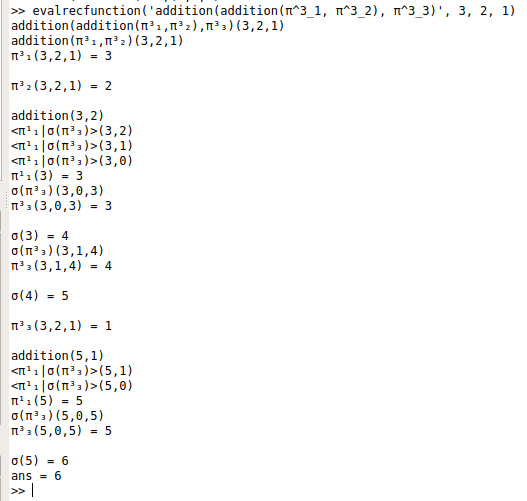
\includegraphics[scale=0.41]{addition3}
\end{center}


\subsubsection*{Ejercicio 3: Implement a WHILE program that computes the sum of three values. You must use an auxiliary variable that accumulates the result of the sum}

\whileprogram{Q}{3,3}{}{S}
\begin{whilecode}[H]
 	\While{$X_2 \not = 0$}{
  	$X_1 \Assig X_1 + 1$\;
  	$X_2 \Assig X_2 -1$\;
	}
	\While{$X_3 \not = 0$}{
  	$X_1 \Assig X_1 + 1$\;
  	$X_3 \Assig X_3 -1$\;
  	}
\end{whilecode}

\end{document}

